\section{Introduction To Project} 
\noindent Automated Building Drawing is a project for creating two-dimensional drawings. The main purpose or objective of the project is to make it usable even by the layman. The main target users are the Civil Engineers who want their plans to be printed on the sheets. As of now, they have to create the drawings with the use of paper and pencil. So to automate converting a particular drawing model to the print ready drawings, this project will be beneficial. The interface should be easy
to use and pretty intuitive. Because the interface is a thing that makes user experience better and to make the user use it.
The Drawing module allows you to put your work on computer. That is, to put views of your
models in a 2D window and to insert that window in a drawing, for example a sheet with a border, a wall and a circle and finally print that sheet. 
\section{Technologies Used}
\subsection{C++}
\noindent C++ is one of the most popular programming languages and is implemented on a wide variety of hardware and operating system platforms. As an efficient compiler to native code, its application domains include systems software, application software, device drivers, embedded software, high- performance server and client applications, and entertainment software such as video games. Several groups provide both free and proprietary C++ compiler software, including the GNU Project, Microsoft, Intel and Embarcadero Technologies. C++ has greatly influenced many other
popular programming languages, most notably C\# and Java. Other successful languages such as Objective- C use a very different syntax and approach to adding classes to C.\\

\noindent Bjarne Stroustrup began his work on C with Classes in 1979. The idea of creating a new language originated from Stroustrups experience in programming for his Ph.D. thesis. Stroustrup found that Simula had features that were very helpful for large software development, but the language was too slow for practical use, while BCPL was fast but too low-level to be suitable for large software development. When Stroustrup started working in AT\&T Bell Labs, he had the problem of analyzing the UNIX kernel with respect to distributed computing. Remembering his Ph.D. experience, Stroustrup set out to enhance the C language with Simula-like features. C was chosen because it was general-purpose, fast, portable and widely used. Besides C and Simula, some other languages
that inspired him were ALGOL 68, Ada, CLU and ML. At first, the class, derived class, strong type checking, inlining, and default argument features were added to C via Stroustrups C++ to C compiler, Cfront. The first commercial implementation of C++ was released on 14 October 1985.

\subsection{Introduction To Qt}
\noindent Qt Creator is a complete IDE for creating applications with Qt Quick and the Qt application framework. Qt is designed for developing applications and user interfaces once and deploying them across several desktop and mobile operating systems. One of the major advantages of Qt Creator is that it allows a team of developers to share a project across different development platforms (Microsoft Windows, Mac OS X, and Linux) with a common tool for development and debugging.
In addition, UI designers can join the team by using Qt Quick tools for creating fluid user interfaces in close cooperation with the developers. The main goal for Qt Creator is meeting the development needs of Qt Quick developers who are looking for simplicity, usability, productivity, extendibility and openness, while aiming to lower the barrier of entry for newcomers to Qt Quick and Qt. The key features of Qt Creator allow UI designers and developers to accomplish the following tasks:
\begin{itemize}
\item Get  started  with  Qt  Quick  application  development  quickly  and  easily  with  examples,  tutorials,
and project wizards.
\item Design  application  user  interface  with  the  integrated  editor,  Qt  Quick  Designer,  or  use graphics
software to design the user interface and use scripts to export the design to Qt Quick Designer.
\item Develop  applications   with  the   advanced  code  editor  that  provides  new  powerful  features  for
copleting code snippets, refactoring code, and viewing the element hierarchy of QML files.
\item Build  and  deploy  Qt  Quick  applications  that  target  multiple  desktop and mobile platforms, such
as Microsoft Windows, Mac OS X, Linux, Symbian, MeeGo, and Maemo.
\item Debug  JavaScript  functions  and  execute  JavaScript  expressions  in  the  current  context,   and
inspect QML at runtime to explore the object structure, debug animations, and inspect colors.
\item Profile  your  Qt  Quick  applications  with  the  QML  Profiler.  You can inspect binding evaluations,
signal  handling,  and  painting  operations  when  running  QML  code.  This  is  useful  for  identifying
potential bottlenecks, especially in the evaluation of bindings.
\item Deploy  applications  to  mobile  devices  and  create  application  installation  packages  for  Symbian
and Maemo devices that can be published in the Ovi Store and other channels.
\item Easily access information with the integrated context­sensitive Qt Help system.
\item It has differents modes such as Welcome, edit debug, design,analyze and help
\end{itemize}
\subsection{libdxfrw}
\noindent libdxfrw is a free C++ library to read and write DXF files in both formats, ascii and binary form. It is licensed under the terms of the GNU General Public License version 2 (or at you option any later version).
\subsection*{Building and installing the library}
mkdir build\\
cd build\\
cmake ..\\
make \\
sudo make install
\subsection*{For non-debug version}
mkdir release\\
cd release\\
cmake -DCMAKE\_BUILD\_TYPE=Release ..\\
make \\
sudo make install
\subsection*{For UBUNTU/Mint Folks}
mkdir release\\
cd release\\
 cmake - DCMAKE\_BUILD\_TYPE=Release -DCMAKE\_INSTALL\_PREFIX:PATH=/usr .. \&\& make all\\
make \\
sudo make install

\subsection{Introduction to GitHub}
\noindent GitHub is a Git repository web-based hosting service which offers all of the functionality of Git as well as adding many of its own features. Unlike Git which is strictly a command-line tool, Github provides a web-based graphical interface and desktop as well as mobile integration. It also provides access control and several collaboration features such as wikis, task management, and bug tracking and feature requests for every project.\\

\noindent GitHub offers both paid plans for private repto handle everything from small to very large projects with speed and efficiency. ositories, and free accounts, which are usually used to host open source software projects. As of 2014, Github reports having over 3.4 million users, making it the largest code host in the world.\\

\noindent GitHub has become such a staple amongst the open-source development community that many developers have begun considering it a replacement for a conventional resume and some employers require applications to provide a link to and have an active contributing GitHub account in order to qualify for a job.

\subsection{What is Git?}
\noindent Git is a distributed revision control and source code management (SCM) system with an emphasis on speed, data integrity, and support for distributed, non-linear workflows. Git was initially designed and developed by Linus Torvalds for Linux kernel development in 2005, and has since become the most widely adopted version control system for software development.\\

\noindent As with most other distributed revision control systems, and unlike most client–server systems, every Git working directory is a full-fledged repository with complete history and full version-tracking capabilities, independent of network access or a central server. Like the Linux kernel, Git is free and open source software distributed under the terms of the GNU General Public License version 2 to handle everything from small to very large projects with speed and efficiency.\\

\noindent Git is easy to learn and has a tiny footprint with lightning fast performance. It outclasses SCM tools like Subversion, CVS, Perforce, and ClearCase with features like cheap local branching, convenient staging areas, and multiple workflows.

\subsection{Installation of Git}

Installation of git is a very easy process.
The current git version is: 2.0.4.
Type the commands in the terminal:\\\\
\emph{
\$ sudo apt-get update\\\\
\$ sudo apt-get install git\\\\}
This will install the git on your pc or laptop.

\subsection{Various Git Commands}

Git is the open source distributed version control system that facilitates GitHub activities on your laptop or desktop. The commonly used Git command line instructions are:-\\

\subsection*{Create Repositories}
\addcontentsline{toc}{subsection}{Create Repositories}
Start a new repository or obtain from an exiting URL

\begin{description}

\item [\$ git init [ project-name]]\\
Creates a new local repository with the specified name
\item [\$ git clone [url]]\\
Downloads a project and its entire version history

\end{description}


\subsection*{Make Changes}
\addcontentsline{toc}{subsection}{Make Changes}
Review edits and craft a commit transaction

\begin{description}

\item [\$ git status] \leavevmode \\
Lists all new or modified files to be committed

\item [\$ git diff] \leavevmode \\
Shows file differences not yet staged

\item [\$ git add [file]]\\
Snapshots the file in preparation for versioning

\item [\$ git reset [file]]\\
Unstages the file, but preserve its contents

\item [\$ git commit -m "[descriptive message]"]\\
Records file snapshots permanently in version history

\end{description}

\section{Introduction to \LaTeX}
\begin{figure}[ht]
\centering

\includegraphics[scale=0.2]{images/latex.png}
\caption{\LaTeX{} Logo}
\end{figure}
\hspace{-1.8em} \LaTeX{}, I had never heard about this term before doing this project,
but when I came to know about it's features, it is just excellent. 
\LaTeX (pronounced /ˈleɪtɛk/, /ˈleɪtɛx/, /ˈlɑːtɛx/, or /ˈlɑːtɛk/) is a 
document markup language and document preparation system for the \TeX{} 
typesetting  program. Within the typesetting system, its name is styled 
as \LaTeX.
\begin{figure}[ht]
\centering
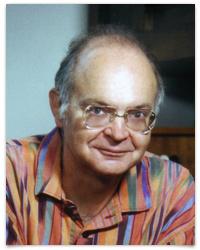
\includegraphics[scale=0.4]{images/donald.jpg}
\caption{Donald Knuth, Inventor Of \TeX{} typesetting system}
\end{figure}

\hspace{-1.8em} Within the typesetting system, its name is styled as \LaTeX. The term 
\LaTeX{} refers only to the language in which documents are written, 
not to the editor used to write those documents. In order to create a 
document in \LaTeX, a .tex file must be created using some form of text 
editor. While most text editors can be used to create a \LaTeX{} document, 
a number of editors have been created specifically for working with \LaTeX.\\

\noindent\LaTeX{} is most widely used by mathematicians, scientists, 
engineers, philosophers, linguists, economists and other scholars in 
academia. As a primary or intermediate format, e.g., translating DocBook 
and other XML-based formats to PDF, \LaTeX{} is used because of the 
high quality of typesetting achievable by \TeX. The typesetting system 
offers programmable desktop publishing features and extensive facilities 
for automating most aspects of typesetting and desktop publishing, 
including numbering and cross-referencing, tables and figures, 
page layout and bibliographies.\\

\noindent\LaTeX{} is intended to provide a high-level language that
accesses the power of \TeX. \LaTeX{} essentially comprises a
collection of \TeX{} macros and a program to process \LaTeX documents. 
Because the \TeX{} formatting commands are very low-level, it is usually 
much simpler for end-users to use \LaTeX{}.


\subsection{Typesetting}
\LaTeX{} is based on the idea that authors should be able to focus on 
the content of what they are writing without being distracted by its 
visual presentation. in preparing a \LaTeX{} document, the author 
specifies the logical structure using familiar concepts such as 
chapter, section, table, figure, etc., and lets the \LaTeX{} system 
worry about the presentation of these structures. it therefore 
encourages the separation of layout from content while still allowing 
manual typesetting adjustments where needed. 

\begin{verbatim}
\documentclass[12pt]{article}
\usepackage{amsmath}
\title{\LaTeX}
\begin{document}
  \maketitle 
  \LaTeX{} is a document preparation system 
  for the \TeX{} typesetting program.
   \par 
   $E=mc^2$
\end{document}
\end{verbatim}

\subsection{Installing \LaTeX{} on System}
Installation of \LaTeX{} on personal system is quite easy. As i have used \LaTeX{} on Ubuntu 13.04 so i am discussing the installation steps for Ubuntu 13.04 here:
\begin{itemize}
\item Go to terminal and type\\\\
\textit{sudo apt-get install texlive-full}
\item Your Latex will be installed on your system and you can check for manual page by typing.\\\\
\textit{man latex}\\

in terminal which gives manual for latex command.
\item To do very next step now one should stick this to mind that the document which one is going to produce is written in any type of editor whether it may be your most common usable editor Gedit or you can use vim by installing first vim into your system using command.\\\\
\textit{sudo apt-get install vim}
\item After you have written your document it is to be embedded with some set of commands that Latex uses so as to give a structure to your document. Note that whenever you wish your document to be looked into some other style just change these set of commands.
\item When you have done all these things save your piece of code with .tex format say test.tex. Go to terminal and type\\\\
\textit{latex path of the file test.tex Or pdflatex path of the file test.tex\\ eg: pdflatex test.tex}\\
for producing pdf file simultaneously.\\
After compiling it type command\\\\
\textit{evince filename.pdf\\ eg: evince test.pdf}\\
To see output pdf file. 
\end{itemize}

\subsection{Making Graphics in \LaTeX{}}
\LaTeX{} s also know popularly for making complex graphics. One such example is shown below here:\\
\begin{verbatim}
\documentclass{article}
\usepackage{tikz}
\usetikzlibrary{calendar,shadings}
\renewcommand*{\familydefault}{\sfdefault}
\colorlet{winter}{blue}
\colorlet{spring}{green!60!black}
\colorlet{summer}{orange}
\colorlet{fall}{red}
\newcount\mycount
\begin{document}
\begin{tikzpicture}[transform shape,
every day/.style={anchor=mid,font=\tiny}]
\node[circle,shading=radial,outer color=blue!30,inner color=white,
minimum width=15cm] {\textcolor{blue!80!black}{\Huge\the\year}};
\foreach \month/\monthcolor in
{1/winter,2/winter,3/spring,4/spring,5/spring,6/summer,
7/summer,8/summer,9/fall,10/fall,11/fall,12/winter} {
\mycount=\month
\advance\mycount by -1
\multiply\mycount by 30
\advance\mycount by -90
\shadedraw[shading=radial,outer color=\monthcolor!30,middle color=white,
inner color=white,draw=none] (\the\mycount:5.4cm) circle(1.4cm);
\calendar at (\the\mycount:5.4cm) [
dates=\the\year-\month-01 to \the\year-\month-last]
if (day of month=1) {\large\color{\monthcolor!50!black}\tikzmonthcode}
if (Sunday) [red]
if (all) {
\mycount=1
\advance\mycount by -\pgfcalendarcurrentday
\multiply\mycount by 11
\advance\mycount by 90
\pgftransformshift{\pgfpointpolar{\mycount}{1.2cm}}};}
\end{tikzpicture}
\end{document}
\end{verbatim}\\
%\begin{figure}[ht]
%\centering
%\includegraphics[scale=0.4]{images/3d.png}
%\caption{Graphics in \LaTeX{}}
%\end{figure}
\LaTeX{} with just invoking few additional packages.

\subsection{Pdfscreen \LaTeX{}}
There are some packages that can help to have unified document using \LaTeX{}. Example of such a package is pdfscreen that let the user view it’s document in two forms-print and screen. Print for hard copy and screen for viewing your document on screen. Download this package from www.ctan.org/tex-archive/macros/latex/contrib/pdfscreen/.\\
Then install it using above mention method.\\

\noindent To test it the test code is given below:-\\
Just changing print to screen gives an entirely different view. But for working of pdfscreen another package required are comment and fancybox.\\

\noindent The fancybox package provides several different styles of boxes for framing and rotating content in your document. Fancybox provides commands that produce square-cornered boxes with single or double lines, boxes with shadows, and round-cornered boxes with normal or bold lines. You can box mathematics, floats, center, flushleft, and flushright, lists, and pages.\\
 	
\noindent Whereas comments package selectively include/excludes portions of text. The comment package allows you to declare areas of a document to be included or excluded. One need to make these declarations in the preamble of your file. The package uses a method for exclusion that is pretty robust, and can cope with ill-formed bunches of text.\\

\noindent So these extra packages needed to be installed on system for the proper working of pdfscreen package.
\section{Web based graphic generation using \LaTeX{}}
\LaTeX{} is also useful when there is need of generating the graphics from browser. For
example to draw a circle by just entering its radius in html input box. So this kind
A
of project can be conveniently handled using \LaTeX{}. Basic idea behind this generation
process is that when user clicks on submit button after entering radius a script will run
that enter the radius in already made .tex file and recompiles it on server and makes its
pdf and postscript file. After that user can view those files by clicking on link provided
to view the files. See some screen shots of such a graphic generation project made by
Dr. H.S. Rai:\\
So here in the above input page which is also the index page user can enter input
for length of rectangle, breadth of rectangle and for radius of circle after that user can submit the values. After the values get submitted a script get runs by php code at server
side. This script first enters the dimensions of rectangle and circle that were selected by
user in to an already existing .tex file and replace with the older dimensions there. After
that script recompiles the the tex file and make it available for user.\\
	
\noindent In above figure it gets clear that .tex file has been compiled and pdf and postscript files
are available to user and user can download the graphics so produced. Hence graphics
can be generated in \LaTeX{} through web interface.

\section{Objectives}
\begin{itemize}
\item To put views of your models in a 2D window and to insert that window in a drawing.
\item To increase the productivity and hence efficiency.
\item To encourage civil engineers to use the computer instead of drawing sheets.
\item To create the drawings of various entities without using the mouse.
\item To eliminate manual operations and thus saving the time and money by automating the entire drawing process.
\end{itemize}
